  
\chapter{Results}
To test the software, the two stations were situated one outside the Electric and Electronic labs at Stellenbosch University and the other inside, with the UART giving the output as follows:
\definecolor{mygreen}{rgb}{0,0.6,0}
\definecolor{mygray}{rgb}{0.5,0.5,0.5}
\definecolor{mymauve}{rgb}{0.58,0,0.82}
\definecolor{terminalbgcolor}{HTML}{330033}
\definecolor{terminalrulecolor}{HTML}{000099}
\lstset{
	backgroundcolor=\color{terminalbgcolor},
	basicstyle=\color{white}\fontfamily{fvm}\footnotesize\selectfont,
	breakatwhitespace=false,  
	breaklines=true,
	captionpos=b,
	commentstyle=\color{mygreen},
	deletekeywords={...},
	escapeinside={\%*}{*)},
	extendedchars=true,
	frame=single,
	keepspaces=true,
	keywordstyle=\color{blue},
	%language=none,
	morekeywords={*,...},
	numbers=none,
	numbersep=5pt,
	framerule=2pt,
	numberstyle=\color{mygray}\tiny\selectfont,
	rulecolor=\color{terminalrulecolor},
	showspaces=false,
	showstringspaces=false,
	showtabs=false,
	stepnumber=2,
	stringstyle=\color{mymauve},
	tabsize=2
}
\begin{figure}[!htb]
\begin{lstlisting}
Bytes received: 80
SATELLITE time: 2023/5/16-21:55:57 Location: -33.9286628330, 18.8670256670 CO2:  +469.00,
MassConcentrationPm1p0:  +3.60,MassConcentrationPm2p5: 3.80,MassConcentrationPm4p0: 3.80,
MassConcentrationPm10p0: 3.80,AmbientHumidity: 86.72,AmbientTemperature: 10.62C,
VocIndex: 19.00,NoxIndex: 1.00
\end{lstlisting}
\end{figure}

\noindent
This shows the received contents from the satellite station, as well as the size of the bytes received. This confirms the transfer system working as expected. With this confirmed, the next test was to see if the WiFi download server was working on the base station and if the data has been written to the SD card.

\begin{figure}[!htb]
	\minipage{0.4\textwidth}%
	\includegraphics[width=\textwidth]{body/fig/ESPServer}
	\caption{Main page for website}
	\label{fig:espserver}
	\endminipage\hfill
	\minipage{0.4\textwidth}%
	\includegraphics[width=\textwidth]{body/fig/datacsvshow}
	\caption{data.csv file present on the SD card and accessible through the URL}
	\label{fig:datacsvshow}
	\endminipage\hfill
\end{figure}

\noindent
From Figure~\ref{fig:datacsvshow} it can be seen that the data was accessible from the web portal when connected to the WiFi access point.
\pagebreak

\begin{figure}[!htb]
	\centering
	\includegraphics[width=0.5\linewidth]{body/fig/speed}
	\caption{Speed of download is about 270kB/s }
	\label{fig:speed}
\end{figure}

\noindent
When measuring the speed of the download using the local network, the data was downloaded at about 270 kB/s, this would mean a days data would take about four seconds to download. This means the system is capable of providing data to an outside entity at sufficient speeds should it need to, like a database.


%First say what you are looking at. Then say what yo get from figure
%now given this what does it tell you
%for each table and figure

%\end{figure}
\begin{figure}[!htb]
	\centering
	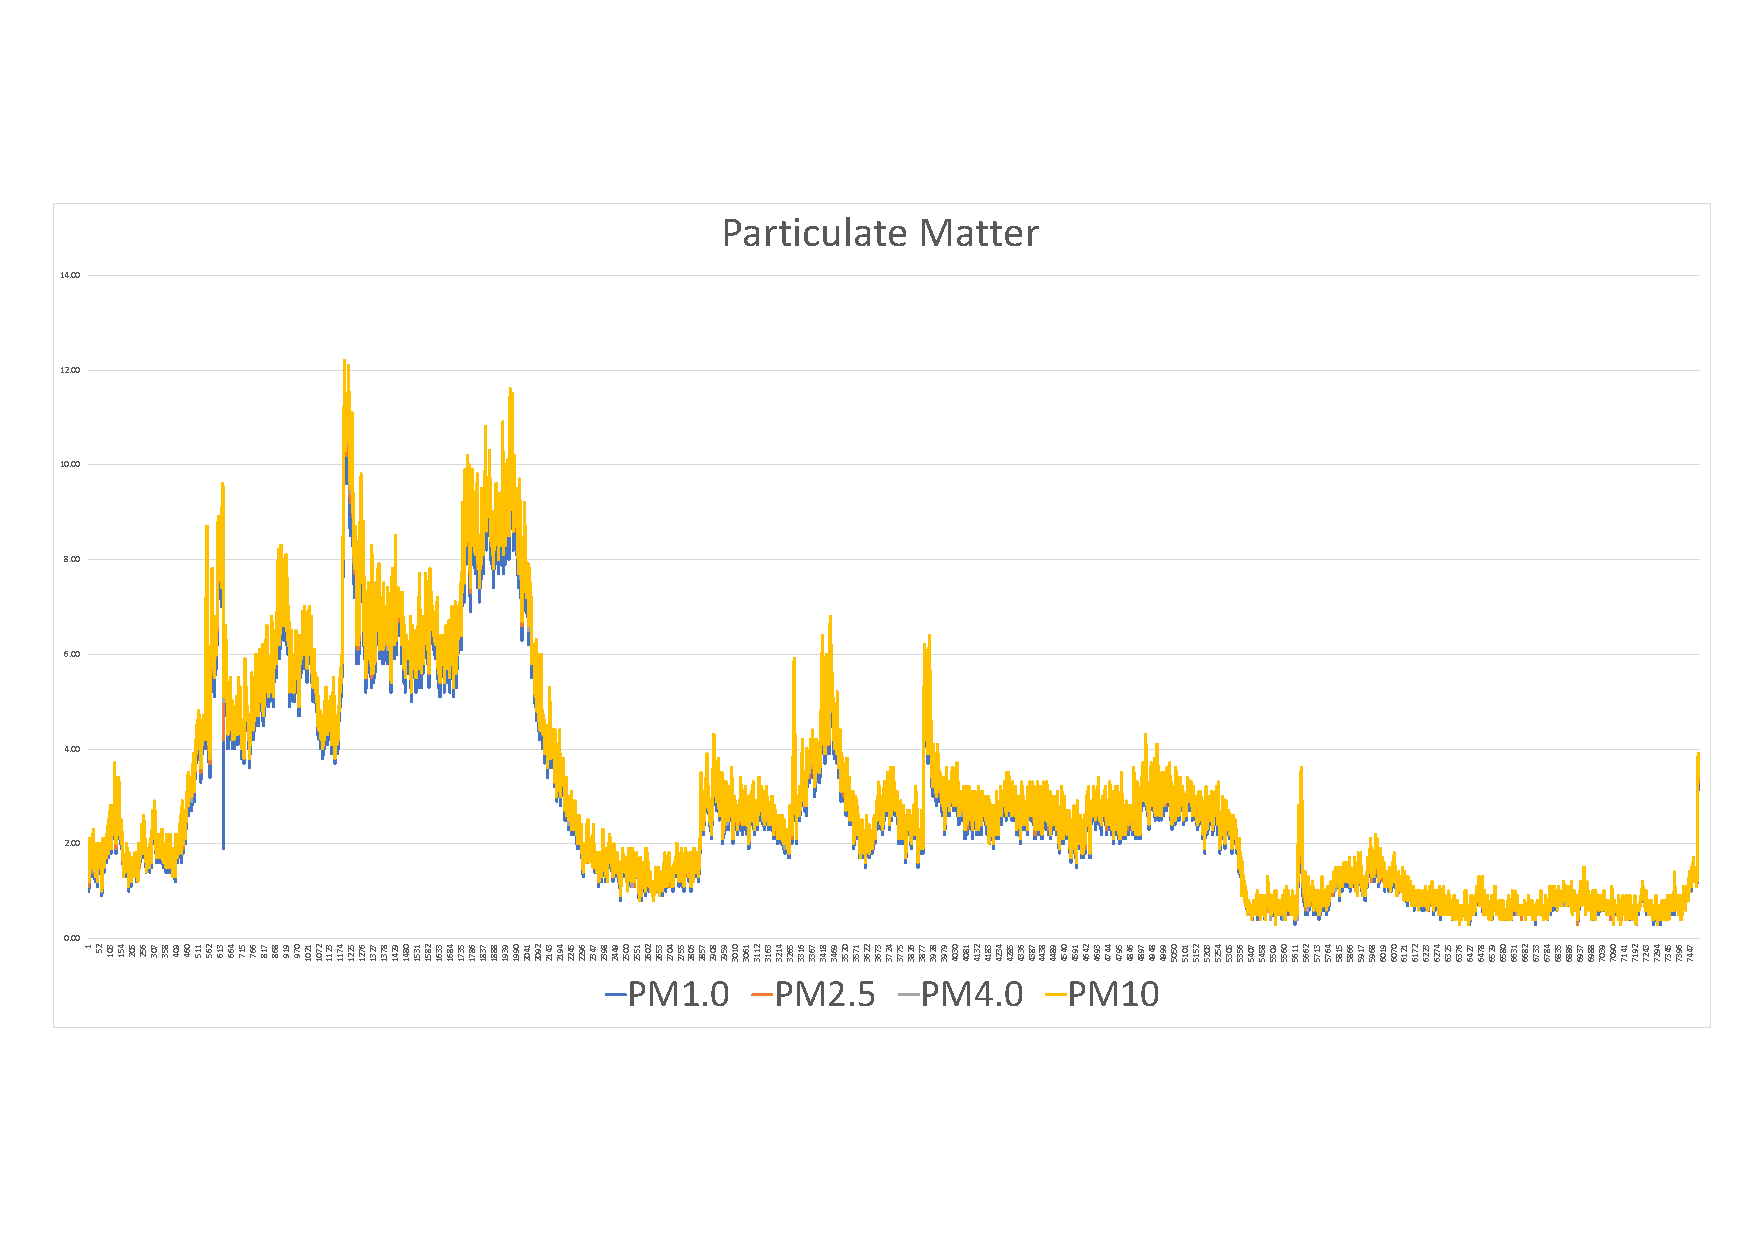
\includegraphics[width=0.9\linewidth]{body/fig/PMall.pdf}
	\caption{Particulate Matter graph of 7000 data points at all concentrations measured.}
	\label{fig:PMall}
\end{figure}

\noindent
The correlation between all of the different sizes of particulate matter concentrations is rather high, as can be seen from Figure~\ref{fig:PMall}, This means we could conceivably only use the PM 2.5 reading as is the norm. The rough timing of the chart is late afternoon to next day, with the elevated period in the middle representing the evening.
The peaks at the start are the testing of the sensor with various methods while it was on my desk.

\pagebreak
\begin{figure}[!htb]
	\centering
	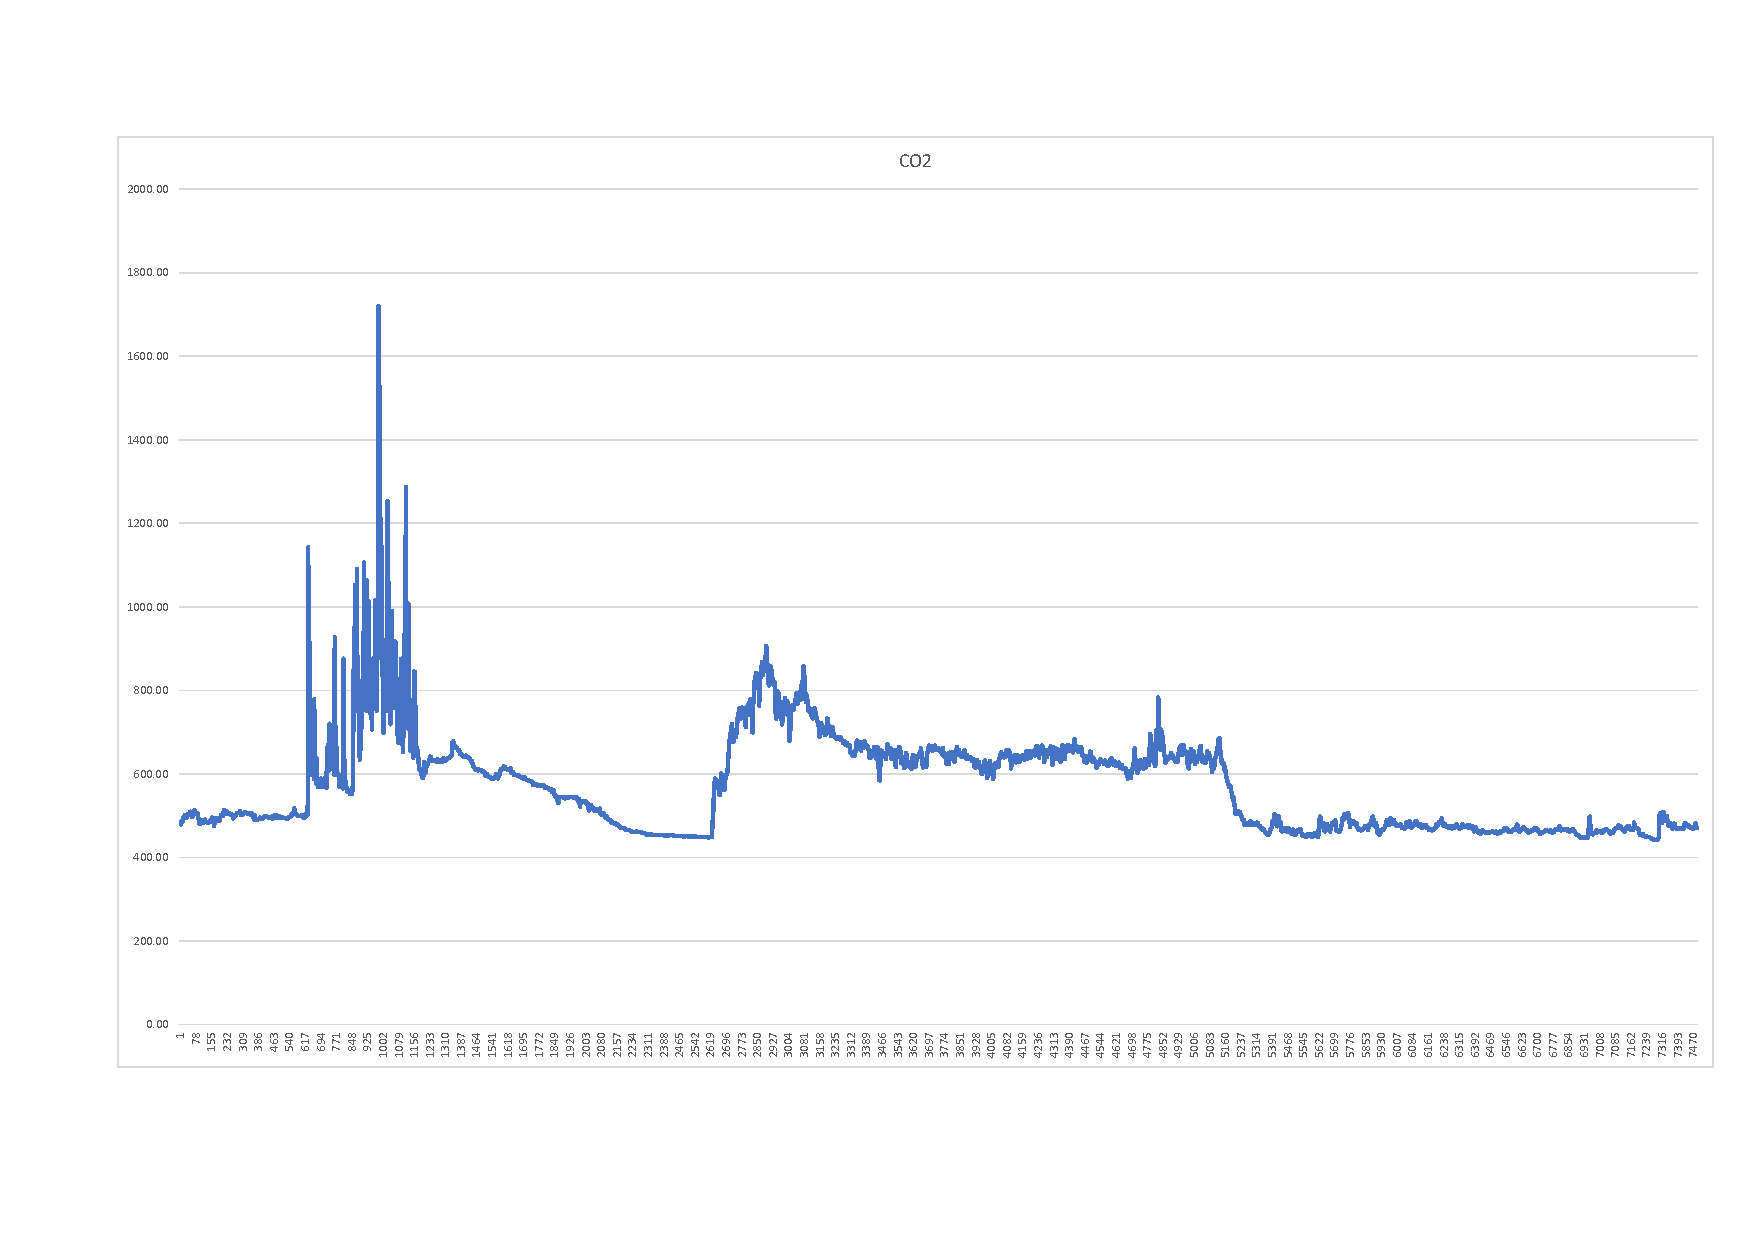
\includegraphics[width=0.7\linewidth]{body/fig/CO2}
	\caption{CO2 measurements}
	\label{fig:co2}
\end{figure}

\noindent
In Figure~\ref{fig:co2} the CO2 concentration is shown for the same time period, here the concentration is much more discernable, with the CO2 remaining consistent and lowering through the night as lighter breathing and less activity realises a slight less steep than the initial start, the dips in-between are when there was no one inside the testing area.


\begin{figure}[!htb]
	\minipage{0.45\textwidth}%
	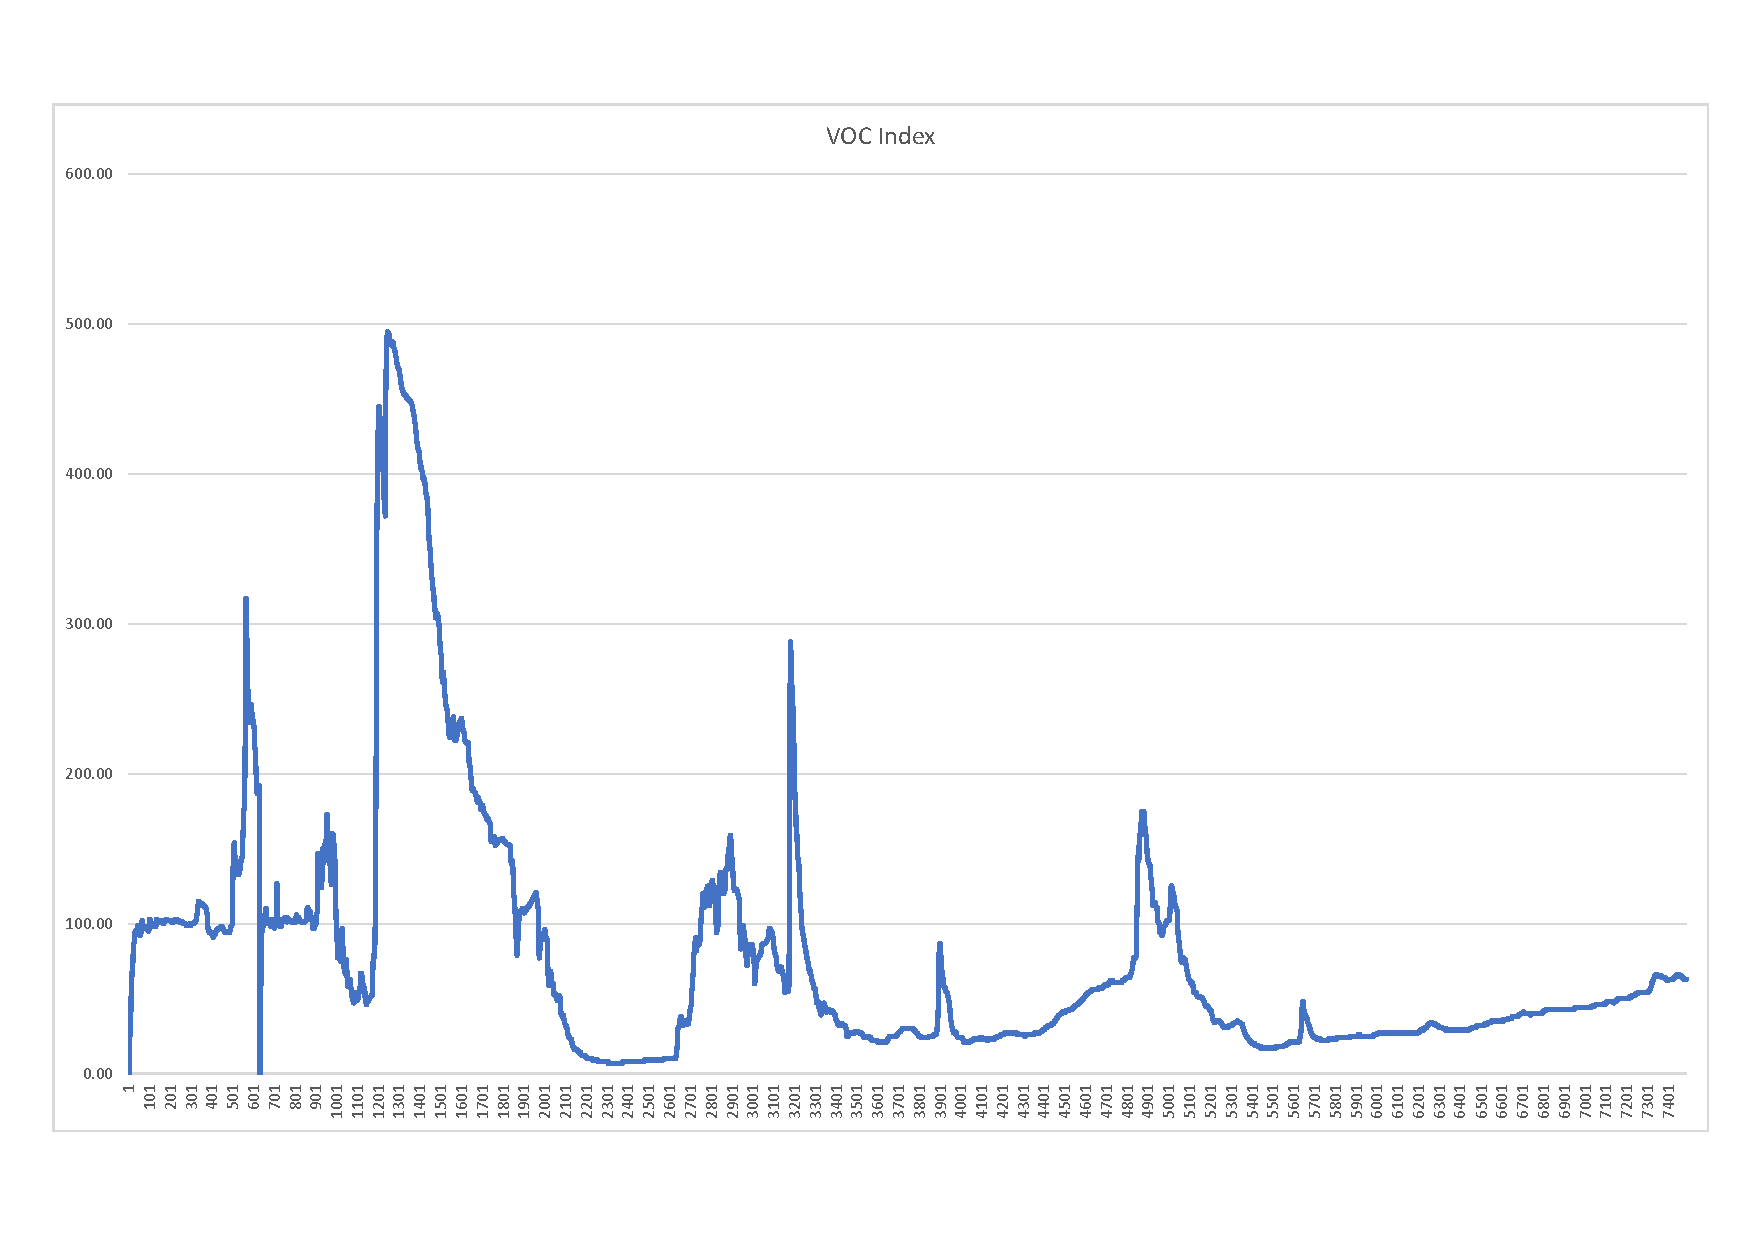
\includegraphics[width=\linewidth]{body/fig/VOC.pdf}
	\caption{VOC}\label{fig:voc}
	\endminipage\hfill
	\minipage{0.45\textwidth}%
	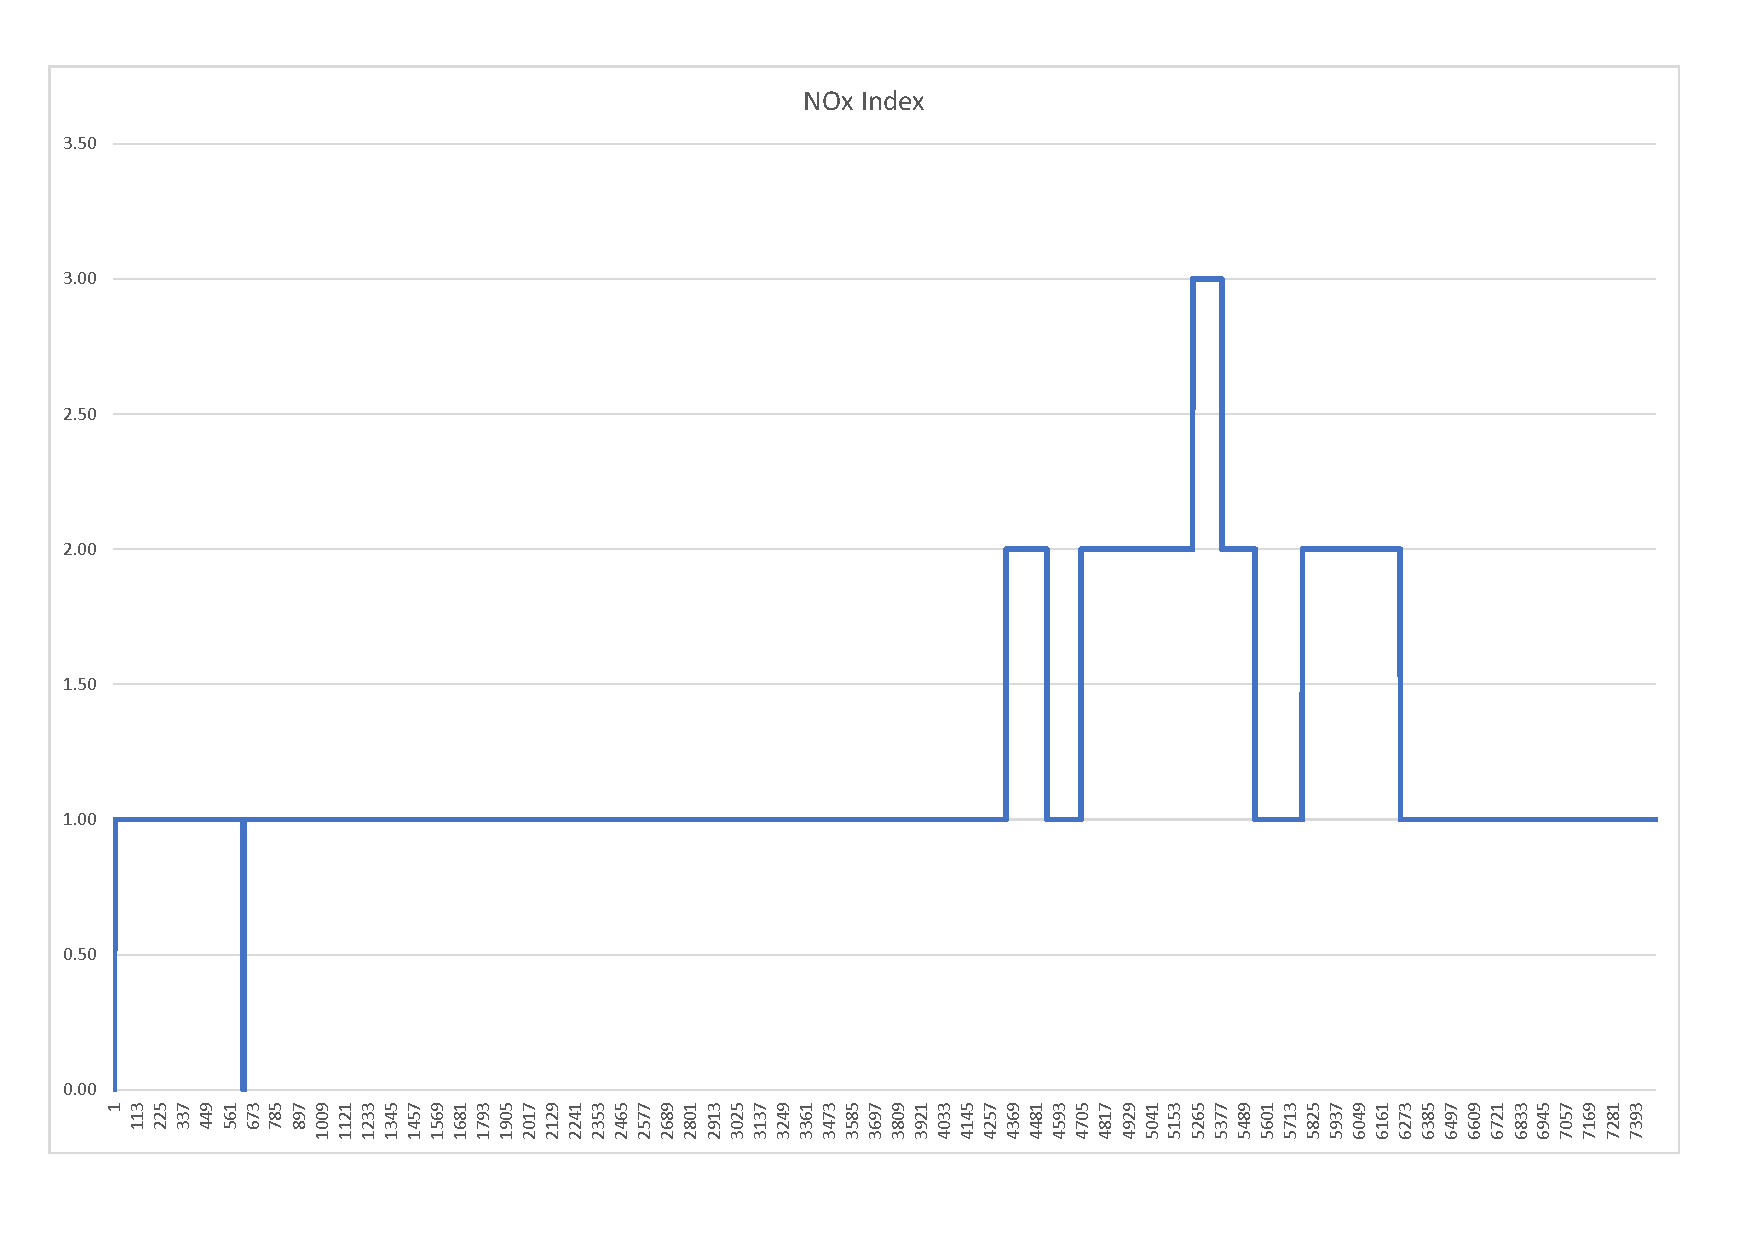
\includegraphics[width=\linewidth]{body/fig/NOX.pdf}
	\caption{NOx}\label{fig:nox}
	\endminipage\hfill

\end{figure}

\noindent
VOC and NOx readings spiked along with the other test samples and as mentioned in the section, the NOx readings only become viable after a few hours, with it also only moving up a few index point, leading the the jagged graph.


%\begin{figure}[!htb]
%	\minipage{0.45\textwidth}%
%	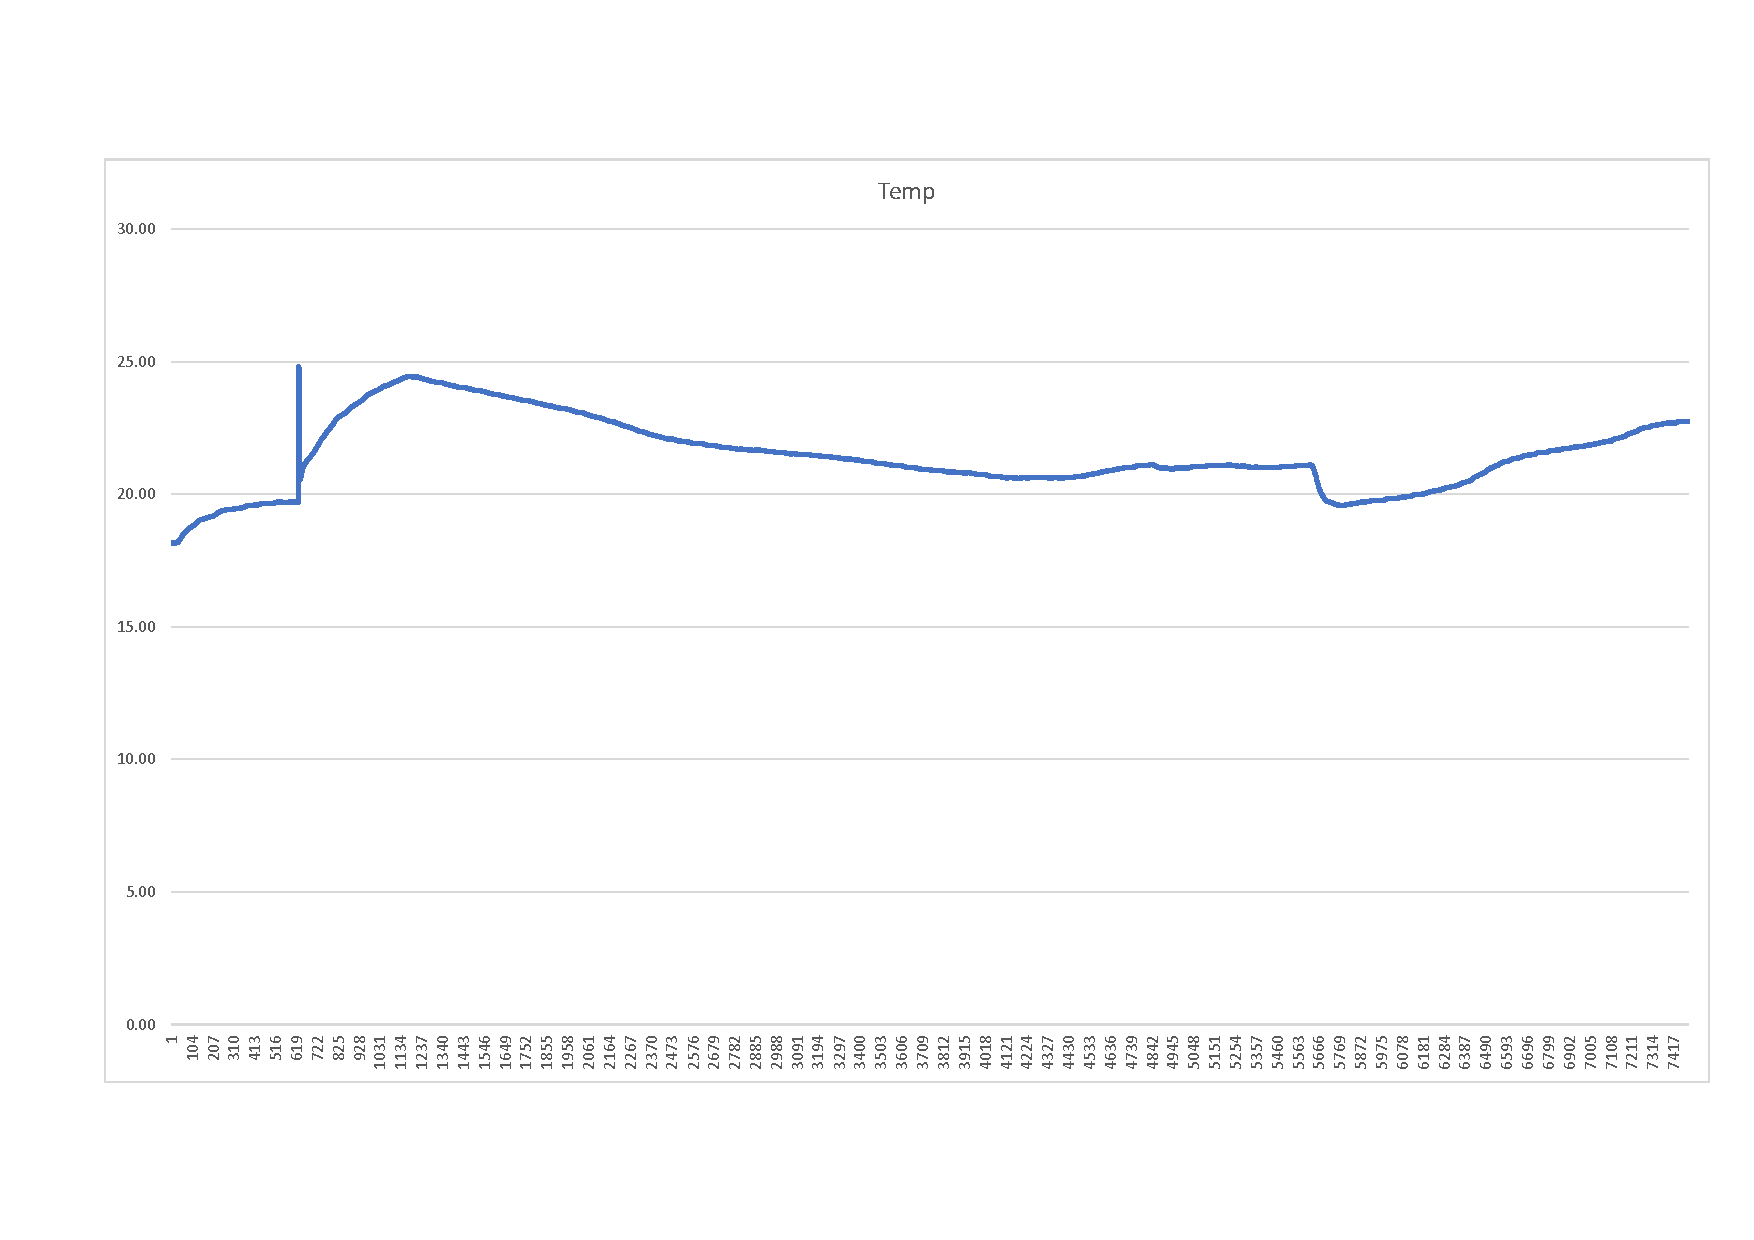
\includegraphics[width=\textwidth]{body/fig/Temp.pdf}%
%	\caption{Temperature}
%	\label{fig:temp}
%	\endminipage\hfill
%	\minipage{0.45\textwidth}%
%	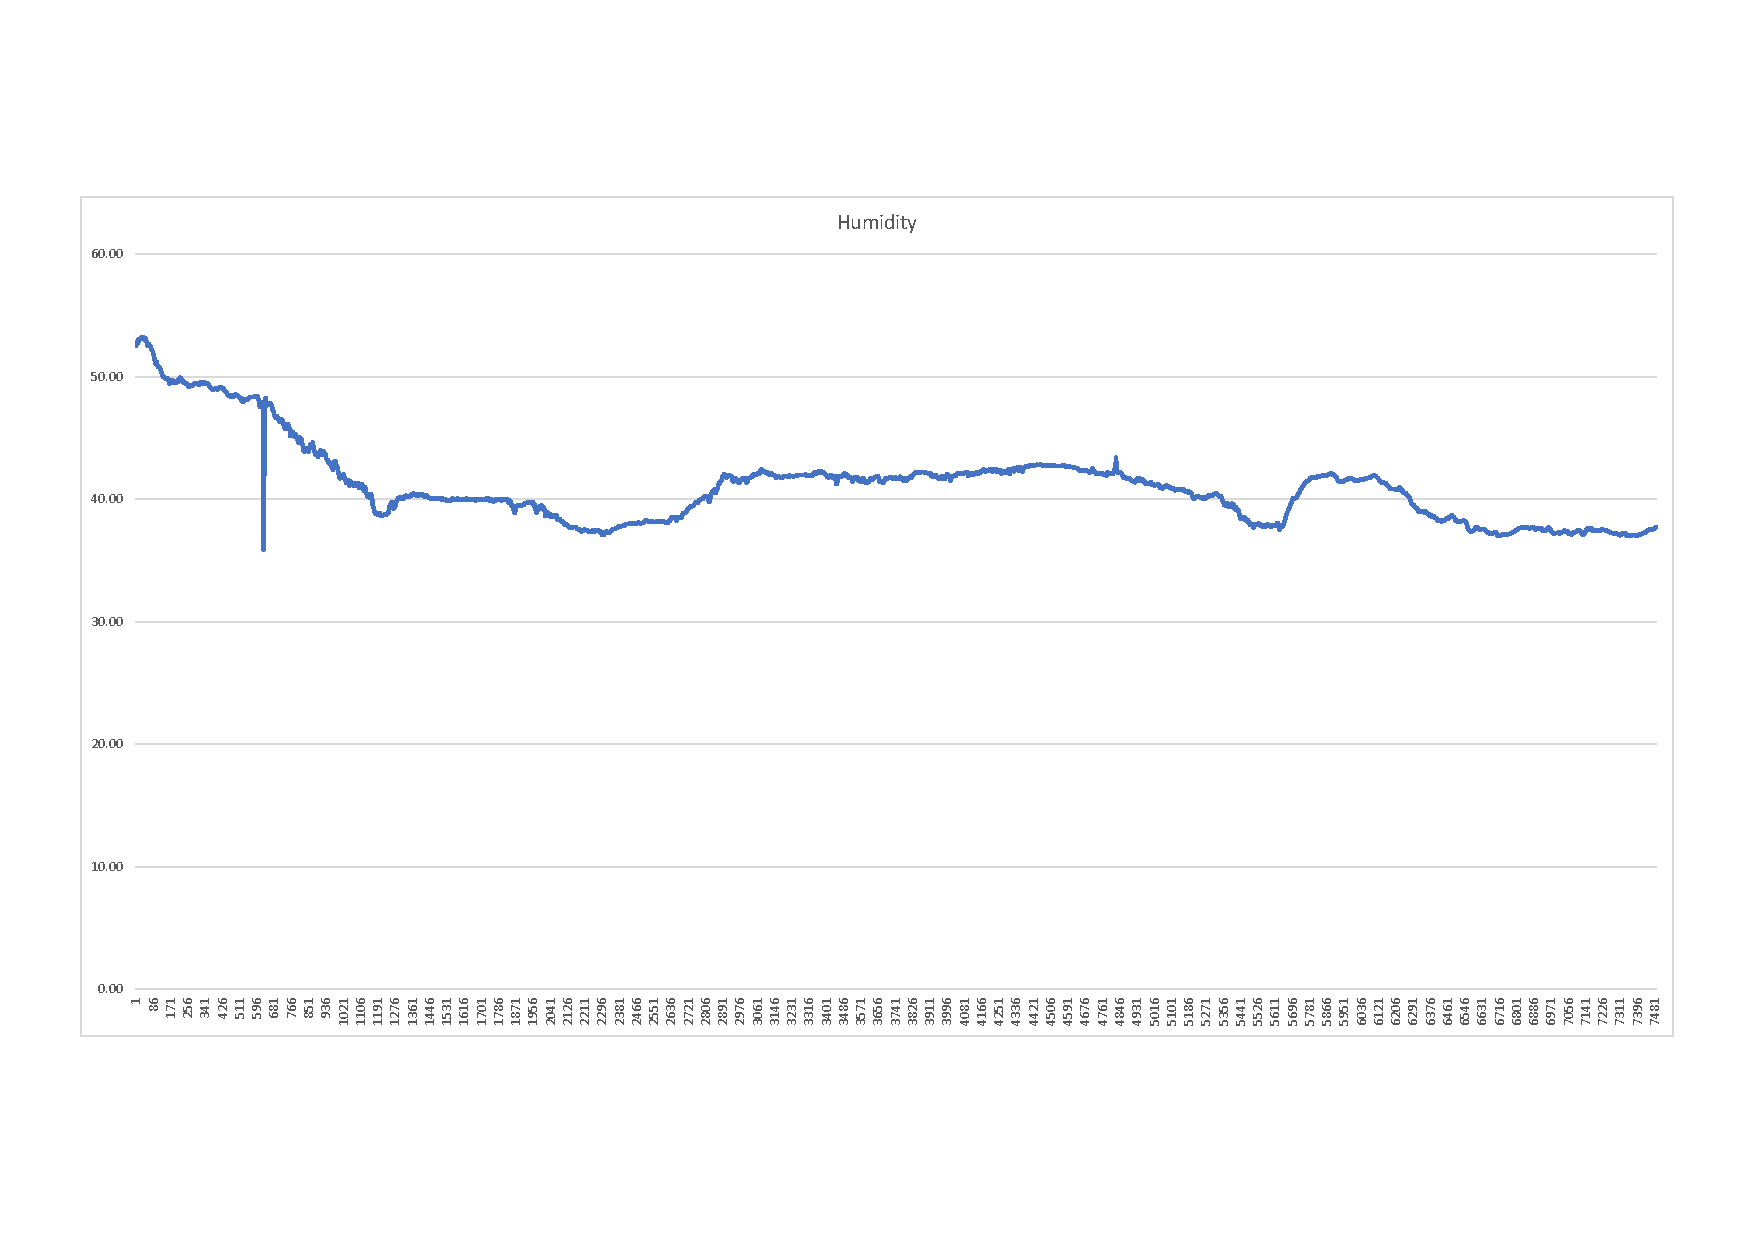
\includegraphics[width=\textwidth]{body/fig/hum.pdf}%
%	\captionof{figure}{Humidity}
%	\label{fig:hum}
%	\endminipage\hfill
%	
%	%\text{Charts provided by \cite{2007Comparison}}
%\end{figure}